\chapter{Converting Vector Spaces into Interpretable Representations}\label{Chapter3}


\section{Introduction}\label{chapter3:Introduction}
%What is the importance of similarit
The ever more pervasive digital infrastructure that supports our lives has resulted in many opportunities to obtain data and models to make sense of that data. Semantic Spaces that encode semantic relationships between documents spatially have recently achieved strong results on tasks like X, Y, Z. These neural-network learned representations make use of a variety of new information like grammatical structure, word-context and even image data. Further, as domains become more entrenched in the digital world, the need for models in safety critical domains like medicine or legal domains like credit evaluation have increased the need for producing interpretable models, as well as interpretable representations. However, the dimensions of a semantic space do not correspond to human understandable features, and standard approaches to interpretable text representations do not match the performance of these methods. Ideally, we would obtain a representation that makes use of the rich semantic relationships from a high-performing semantic space, but also has dimensions corresponding to interpretable features. To this end, we aim to introduce in this chapter a methodology to linearly transform a semantic space using just its associated bag-of-words as input into an interpretable representation, and demonstrate the applicability of this interpretable representation to simple interpretable classifiers. 

There are many types of semantic relationships in a semantic space. For our work, the representation is composed of rankings of documents on semantic directions in the space, in particular where those directions correspond to features. We show an example of the kind-of directions we use to obtain our representation in \ref{ch3:ToyDirectionsGraphic}. Directions from domain-specific semantic spaces have been used previously in a variety of ways, For instance,  \cite{gupta2015distributional} found that features of countries, such as their GDP, fertility rate or even level of CO$_2$ emissions, can be predicted from word embeddings using a linear regression model. Similarly, in \cite{kim2013deriving} directions in word embeddings were found that correspond to adjectival scales (e.g.\ bad $<$ okay $<$ good $<$ excellent) while \cite{DBLP:conf/acl/RotheS16} found directions indicating lexical features such as the frequency of occurrence and polarity of words. 


\begin{figure}[t]
	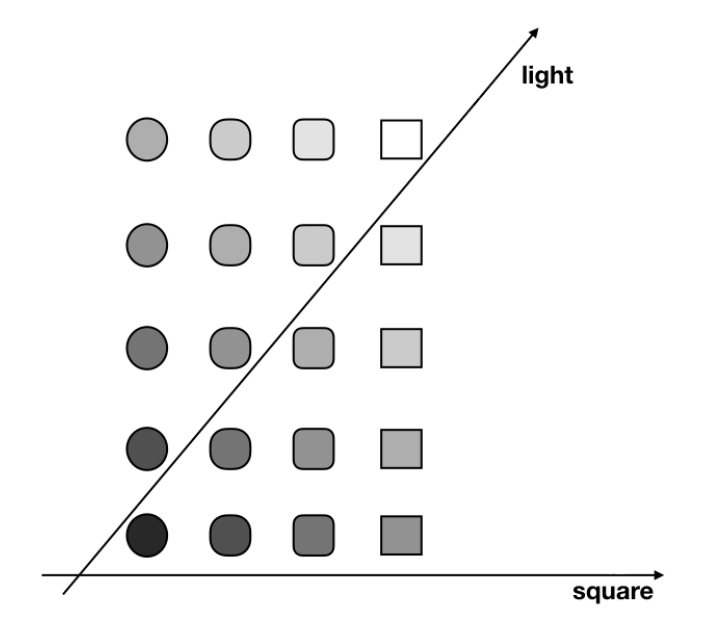
\includegraphics[width=\textwidth]{images/toy_domain.png}
	\centering
	\caption{An example in a toy domain of shapes.}\label{ch3:ToyDirectionsGraphic}
\end{figure}



%Why interpretability for document classification matters:

%What semantic spaces are there that perform well at tasks:

%What document classification tasks are important:

%What methods are there for interpretable document classification:

Derrac \cite{Derrac2015} introduced an unsupervised method to go from a semantic space and its associated bag-of-words to a representation where each dimension is a ranking of documents on a feature of the domain. For example, in the domain of movie reviews genres would be a feature, and the dimension would have a numeric value for each document corresponding to the degree it is a particular genre. The contribution of this Chapter is an analysis and experimentation on the quality of these features applied to document classification. The main insight from our work is that these interpretable features do not suffer a performance drop in a non-linear classifier compared to the original representation, and can outperform the original representation and a baseline interpretable representation in a linear classifier. In addition, we find that if a dimension ranks documents on a feature relevant to the task, it can be competitive with more complex models using a single decision tree node. We show an example of the representation from a domain of IMDB movie reviews in \ref{ch3:TreeAndRep}. 

\begin{figure}[t]
	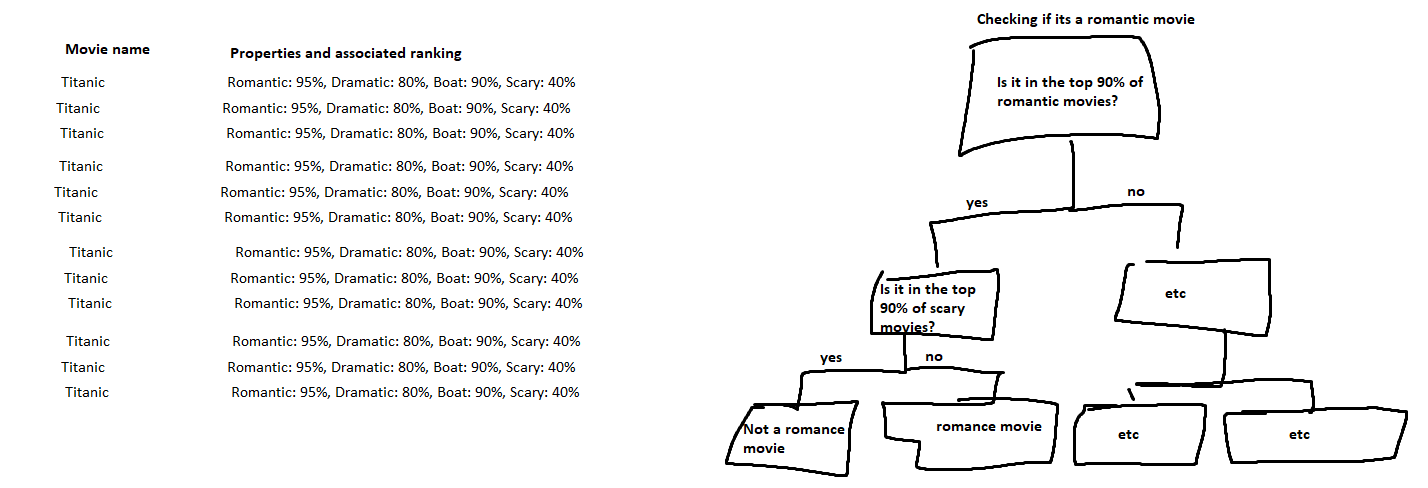
\includegraphics[width=\textwidth]{images/tree and rep.png}
	\centering
	\caption{Example movies and selected associated dimensions, chosen according to their relevance to the genre task.}\label{ch3:TreeAndRep}
\end{figure}

%Semantic spaces encode semantic relationships

%What are the applications of semantic relationships? What is the power of a semantic relationship? Why are semantic relationships important in a space?
%prolly need more about

%What are directions? Why are directions important? What have they been used for? What is a feature direction?


% How can I apply directions to produce an interpretable space? Why is this valuable? What makes this interesting? What are feature rankings?


%%What are the advantages, disadvantages of the previous work?



%Why do this work? What is the value of this work?  How is this relevant to the readers interests?


%\subsection{Using a Property Representation in a Linear Classifier}


%Our method can use any vector space that linearly separates entities, and so it has potential longevity. This means that our method is relying on structure in the space that does not directly correspond to our desired representation -  we can view our approach as a linear transformation of the space. We address this problem in Chapter \ref{chapter:finetuning}. However, we have the capability to leverage many different methods to construct a vector space for our representation, so as long as dense representations of entities exist it will be possible to use our method, and as they are improved the results that our method can achieve will be improved too. This kind of flexibility also gives us the potential to combine the resultant representations from different vector spaces for classification, e.g. concatenating the vectors from different spaces.

%Topic models such as Latent Dirichlet Allocation (LDA) represent documents as multinomial distributions over latent topics, where each of these topics corresponds to a multinomial distribution over words \cite{Blei2003}. These topics tend to correspond to semantically meaningful concepts, hence topic models tend to be rather interpretable \cite{Chang2009}. To characterize the semantic concepts associated with the learned topics, topics are typically labelled with the most probable words according to the corresponding distribution. 

% What is a semantic space? Why is a semantic space valuable?




% 





%%What is the previous work?
 %What is a direction




%Finally, \cite{derracAIJ} found salient properties as direction vectors in a semantic space of entities (e.g. Movies in a domain of IMDB movie reviews), and labelled them with clusters of words (e.g. $p_1 = {Scary, Horror, Gore}, p_2 = {Funny, Laughter, Hilarious}$).  We show a toy example in Figure \ref{ToyDirection}. %Copied from CONLL 




%%What is our contribution towards those disadvantages in this chapter?
 %"Decision Trees, Decision Tables and Textual descriptions of rules are logically equivalent in the sense that one type of representation can be automatically translated to another (albeit in a simpler or more complex form), while preserving the predictive behaviour of the original model"
% has many positive effects for its users, like lower response times \cite{Narayanan2018, Huysmans2011}, better question answering and confidence for logical problem questions \cite{Huysmans2011} and higher satisfaction \cite{Narayanan2018}.


%%What are some real world scenarios that you could see our work taking effect in?
%In a case study by  \cite{Veale2017}, giving the business users the option between a model with higher classification score but more input variables and a lower classification score but less input variables resulted in more buy-in for system designers. By accurately representing salient concepts in the domain, we are also able to offer a similar option; less nodes in the decision tree in exchange for more accuracy. % Potentially this citation sucks


%How is the work evaluated? How can you justify the evaluation? 
%%What are some alternative interpretable classifiers? What are some approaches to interpretable classification?

%%How does our work fit into the niche of interpretable classifiers?

%%What kind of tasks are these interpretable classifiers usually on? How do we compare in terms of evaluation?

%%How does our evaluation of interpretability play into our idea of interpretability outlined in Chapter 1?




%How is the chapter going to play out? Whats going to happen?
%As our work performs well even at lower-depth trees, this gives potential users more flexibility in how they want to present the information, e.g. to a potential client. Compared to bag-of-words, which loses its representation capabilities the lower the depth.

This chapter continues as follows: We begin by describing related work, then explain the method, making explicit the variations we have introduced for our experimental work. We follow this with the results of our experiments accompanied by qualitative examples and explanations, and finish with a conclusion on the  benefits and limitations of this approach.



\section{Related Work}
%Sparse word vectors
%Adapted to composition \cite{Fyshe2015}
\subsection{Semantic Relations \& Their Applications}

Our method uses the relationships inherent in a semantic space. Other work has formalized the relationships found in semantic spaces, for example in word-vectors, linear analogies (see Section \ref{WordVectors, Ethayarajh2018}, were found where the vector between king and queen was parallel to the vector between prince and princess. % NEED TO MAKE THIS REAL
These relationships have been expanded on, for example \cite{TomasMikolovWen-tauYih2013} found that "equivalent relations tended to correspond to parallel vector differences" \cite{Mitchell2015}, and \cite{Mitchell2015}, found that by decomposing representations into orthogonal semantic and syntactic subspaces they were able to produce substantial improvements on various tasks. Additionally, they have also been found to hold inherent gender bias  \cite{Garg2017} as word distances between gendered words (e.g. male, female, she, her) and occupational words e.g. (nurse, programmer) were correlated to the percentage of occupation that gender had for that role in different time periods. %Copy pasted from this 
%[ENTIRE SECTION COPY PASTED FROM PREVIOUS PAPER]
\textbf{Linear Classifiers}
Decision trees, linear SVM's, logistic regression, decision tables, IF Then rules.

What are the available options for interpretable linear classification?

How have each of these methods been measured or validated in the literature in regards to interpretability? How about application to real world situations?

\textbf{Non linear classifiers}
What non linear classifiers networks are interpretable? How have they done it? How have they measured it? How does it compare to a linear method?

\textit {Neural networks}Approximating w/linear model, Interpretable nodes/weights

\textit {Other Stuff}

\subsection{Interpretable Representations}


There are two ways in which topic models can be used for document classification. First, a supervised topic model can be used, in which the underlying graphical model is explicitly extended with a variable that represents the class label \cite{Blei2010}. Second, the parameters of the multinomial distribution corresponding to a given document can be used as a feature vector for a standard classifier, such as a Support Vector Machine (SVM) or Decision Tree. LDA has been extended by many approaches, e.g.\ aiming to avoid the need to manually specify the number of topics \cite{teh2005sharing}, modelling correlations between topics \cite{Blei2006}, or by incorporating meta-data such as authors \cite{rosen2004author} or time stamps \cite{wang2006topics}.


Broadly speaking, in the context of document classification, the main advantage of topic models is that their topics tend to be easily interpretable, while vector space models tend to be more flexible in the kind of meta-data that can be exploited. The approach we propose in this paper aims to combine the best of both worlds, by providing a way to derive interpretable representations from vector space models.

 One of the more popular models for text representation that labels features in a similar way to our method are Topic Models.


\section{Method}
% Assumed understanding at this point
% Chapter 1: Why interpretability is important. The value of a good interpretable representation. What directions are and what they mean.
% Chapter 2: The background and literature review for interpretable representations.
% Chapter 3: An introduction on the value of a good interpretable classifier, and the position of our work in that domain and how it can be applied there. What entities, properties are. What a conceptual space is. A literature review on relevant interpretable classifiers.

This section details the methodology to go from a Bag-Of-Words (BOW) \ref{background:BOW} and Semantic Space \ref{bg:SemanticSpaces}, to rankings of documents on features of the domain, e.g. In a domain of IMDB movie reviews, where a document is composed of all of its reviews, a movie would be ranked on features like ${Scary, Horror, Bloody}$ and ${Romantic, Love, Cute}$, ideally with as many rankings as salient features of the domain. 
%Make sure features ae explained well earlier 

%\subsection{The Structure of a Semantic Space}

%Salient features of the domain are encoded in the structure of a semantic space. 
% What are directions? How are they encoded? Why are they encoded that way?



 %Features that are important will be spatially organized in a way that reflects the similarity between the bag-of-words representations they were composed of. In particular, we expect that documents will be arranged in a direction, where generally the higher the PPMI score for a group of words that correspond to a feature (e.g. $Horror, Scary, Gore$) the further away they will be from those that have low PPMI scores for those words. We give examples of this in Figure \ref{ch3:DirectionsGraphic}, by projecting documents into a 2D space of salient features we are able to show that these documents are structured according to directions for these features. Salient features will typically be a more abstract representation which will be natural in the domain, e.g. in a domain of IMDB movie reviews, genres. 

%\begin{figure}[t]
%%	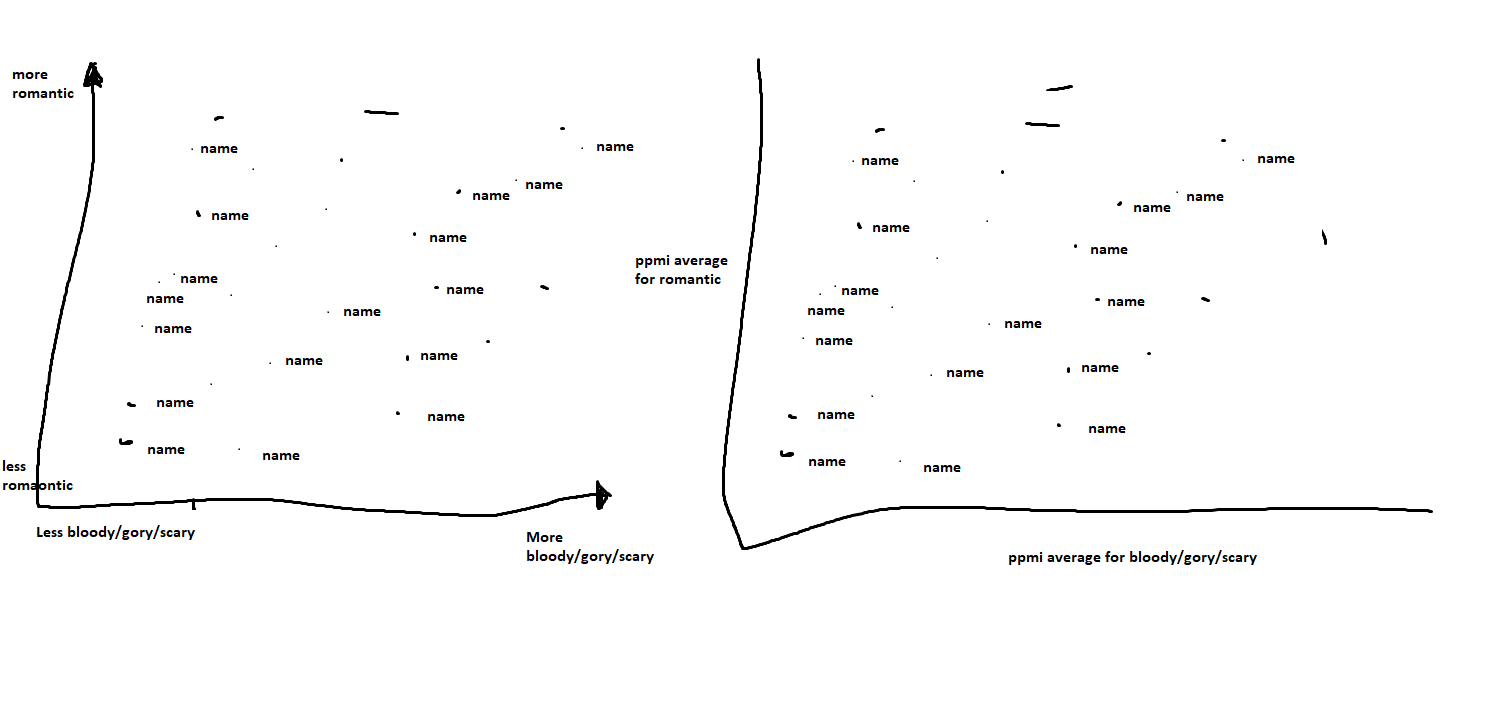
\includegraphics[width=\textwidth]{images/DirectionsGraphic.png}
%	\centering
%	\caption{Original And Converted.}\label{ch3:DirectionsGraphic}
%\end{figure}
%The method to obtain interpretable feature-vectors is an extension of the work by \cite{derracAIJ}. This previous work showed how to, filter out words, cluster words to get features, and obtain rankings of documents on those features. In this section, we further analyse and extend this work, in particular by testing a variety of additional filtering methods and clustering methods, and demonstrating how these feature-vectors can produce simple linear interpretable classifiers. 
%To begin, we filter out terms that will not be well represented in the space, and in-turn will not result in good feature rankings. We do so by first removing all terms below a frequency threshold. Then, for each word we obtain a direction in the space that can induce a ranking of documents on that word, and evaluate how well represented that word is in the space and remove those below a threshold. We can consider the terms remaining to be candidate feature-directions, as they are all well represented in the space and are unlikely to be highly scored as representative due to being infrequent. However, it is possible that they may not represent different information from each other, e.g. "blood" and "bloody" are likely quite similar. Additionally, we can understand that a good feature will not correspond directly to a term, but instead to a more abstract concept, e.g. "Blood, Gore, Horror". To obtain these more abstract feature-directions, and ensure the feature-directions are distinct rather than representing the same information, we cluster together similar feature-directions and obtain their feature-rankings to obtain our final representation. Each of these feature-rankings can be labelled with the cluster of words they are composed of. 



\subsection{Obtaining Directions and Rankings From Words}

In this section we show how to obtain directions for words, and explain how to obtain document representations by ranking documents on these directions. For this step, we do not expect all words to be features of the domain.  In the next sections, we aim to filter these words to obtain salient features.

\noindent \textbf{Obtaining directions for each word} For each word $w$, a Support Vector Machine (See Section \ref{bg:SVM}) classifier is trained on the binary Bag-Of-Words representation of that word, where words are labelled as positive if they occurred more than once $w_f >= 1$ and negative otherwise. Although the separation of documents is binary, we can expect that the degree to which they are classified as the word varies. For example in a space constructed from frequency vectors, we can expect that the documents which contain the word more frequently would be further away from the hyper-plane in the positive direction. Following this, we can consider the vector $v_w$ perpendicular to the hyperplane as the direction that models documents from least relevant at the distance furthest from the hyperplane on the negative side to most relevant for the word $w$ at the distance furthest from the hyperplane at the positive side. We show an example of this in the toy domain in Figure \ref{ch3:ToyHyperPlane}. %Although these directions do formally correspond to vectors, we refer to them as directions to emphasize their intended ordinal meaning: feature directions are aimed at ranking entities rather than e.g.\ measuring degrees of similarity. %Graphical representation of 


\begin{figure}[t]
	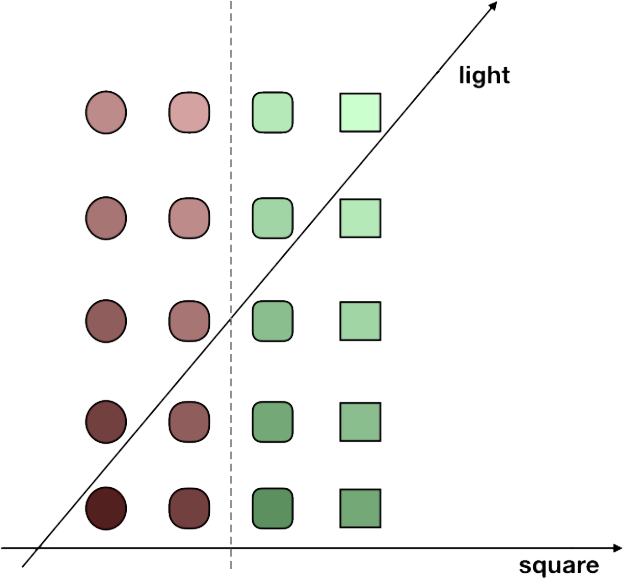
\includegraphics[width=\textwidth]{images/ToyHyperplane.png}
	\centering
	\caption{An example of a hyper-plane and its orthogonal direction in a toy domain of shapes. Green shapes are positive examples and red shapes are negative examples, but despite the problem being binary those closest to the hyper-plane are less defined than those further away, resulting in the orthogonal vector being a direction.}\label{ch3:ToyHyperPlane}
\end{figure}




\noindent \textbf{Ranking documents on directions} Once we have obtained a direction vector for each word $v_w$ the next step is to quantify the degree to which each document has that word, by obtaining a value that corresponds to how far-up it is on the direction vector. These are our rankings of documents on words, if $p_d$ is the representation of a document in the given vector space as a point then we can think of the dot product between the hyper-plane and the document vector $H_w \cdot p_d$ as the ranking $r_dw$ of the document $d$ for the word $w$, and in particular, we take $r_d1 < r_d2$ to mean that $d_2$ has the property labelled with the word $w$ to a greater extent than $e_1$. Below, we show some examples of features and documents ranked on them for different domains. %Graphical representation of entities being ranked on a direction vector






%\begin{figure}[t]
%	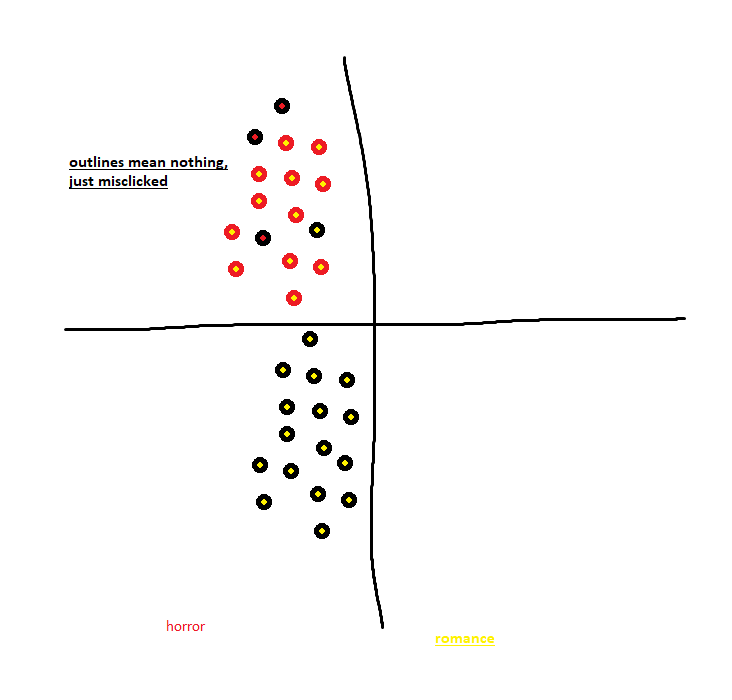
\includegraphics[width=\textwidth]{images/genres_separated.png}
%	\centering
%	\caption{Original And Converted.}\label{ch3:OrigAndConverted}
%\end{figure}



\subsection{Filtering Words}

With the rankings $R_r$, we could create a representation of each document $d$, composed of $w_n$ dimensions, where each dimension is a ranking of the document $d$ on that word $r_dw$. However, many of the words are not spatially important enough in the representation to result in a quality ranking - they are not salient features. In this section, we aim to filter the words that are not separable, we evaluate them using a scoring metric, and remove the words that are not sufficiently well scored. We use three different metrics:

\noindent \textbf{Classification accuracy}. Evaluating the quality in terms of the accuracy of the SVM classifier: if this classifier is sufficiently accurate, it must mean that whether word $w$ relates to document $d$ (i.e.\ whether it is used in the description of $d$) is important enough to affect the semantic space representation of $d$. In such a case, it seems reasonable to assume that $w$ describes a salient property for the given domain.%This is basically copy pasted.
\smallskip

\noindent \textbf{Cohen's Kappa}. One-kind of feature we find in these domains are binary labels of documents, for example a movie either is or isn't a movie with "Gore". We can expect that the more salient a binary feature, the more linearly separable it will be in the space. One problem with accuracy as a scoring function is that these classification problems are often very imbalanced. In particular, for very rare words, a high accuracy might not necessarily imply that the corresponding direction is accurate. For this reason, \cite{Derrac2015} proposed to use Cohen's Kappa score instead. In our experiments, however, we found that accuracy sometimes yields better results, so we retain Kappa as an alternative metric. %This is basically copy pasted.
\smallskip

\noindent \textbf{Normalized Discounted Cumulative Gain} % MATHEMATICS NEEDS TO BE REWRITTEN
This is a standard metric in information retrieval which evaluates the quality of a ranking w.r.t.\ some given relevance scores \cite{jarvelin2002cumulated}.  In our case, the rankings $r_d$ of the document $d$ are those induced by the dot products $v_w \cdot d$ and the relevance scores are determined by the Pointwise Positive Mutual Information (PPMI) score $\textit{ppmi}(w,d)$, of the word $w$ in the BoW representation of entity $d$ where
$\textit{ppmi}(w,d) = \max \big(0, \log\big(\frac{p_{wd}}{p_{w*} \cdotp p_{*d}}\big)\big)$, and
\begin{align*}
p_{wd} &= \frac{n(w, d)}{\sum_{w'} \sum_{d'} n(w', d')}
\end{align*}
where $n(w,d)$ is the number of occurrences of $w$ in the BoW representation of object $d$, $p_{w*} = \sum_{e'} p_{wd'}$ and $p_{*d} = \sum_{w'} p_{w'd}$. %This is basically copy pasted.
\smallskip

By scoring the words on these features, we can apply a simple cut-off (e.g. the top 2000 scored words) to obtain the most salient words. Ideally, this cut-off would be at the point where the words stop corresponding to salient features. However, it is difficult to determine this. In principle, we may expect that accuracy and Kappa are best suited for binary features, as they rely on a hard separation in the space between objects that have the word in their BoW representation and those that do not, while NDCG should be better suited for gradual features. In practice, however, we could not find such a clear pattern in the differences between the words chosen by these metrics despite often finding different words. In Table \ref{Table4}, we show examples of the differences between the largest differences between the scoring methods. % Copy pasted


\subsubsection{Clustering Direction Vectors}

%What are we doing with clustering
If we consider two directions, "Blood" and "Gore", we can understand both of these to be approximating a similar feature of movies, as they both relate to how much blood a movie contains. Because of this, we can expect their directions to be very similar to each other. This is the first idea behind clustering these directions, if we average these directions together we can obtain a direction inbetween them that is a balance between documents that used the word 'Bloody' to describe the blood and the word 'Gore'. To expand on this, some entities would have the property of being bloody films, but did not necessarily use the term gore in their reviews, same as some entities having the property but using the term gore not bloody, we can understand that this new hyper plane and associated direction more accurately represents the property of a bloody film more than either of the terms individually. By extending this to a clustering method, we can find similar abstract features by ensuring that all similar directions are clustered together. %Similarly, obtaining a hyper plane using a Logistic Regression classifier that uses occurences of both and either of these terms as positive would be similar to this averaged direction.

%What is the value of a cluster label?
The word direction for "beautiful" can be nebulous to the interpreter, as it is not clear what it means for a movie to be ranked highly on 'beautiful'. Considering this, clustering provides another advantage, once we cluster the terms to find the property ("beautiful", "cinematography" "shots") we are given context for the word and more easily intuit the feature, in this case it is a feature about how well the movie was directed. 

%The final benefit to clustering the words is that linear classifiers are generally suited better to 'disentangled' representations \cite{Bengio2012}. In this case, we refer to disentanglement in the sense of obtaining a feature vector where each dimension is distinct, rather than the semantic space being naturally clustered. Additionally, if our representation is dense and disentangled into the natural features of the domain, it is unlikely to overfit and will be able to generalize more easily. 

We approach clustering the directions with a variety of methods:

\noindent \textbf{K-Means} K-Means is a clustering algorithm that starts with determining the amount of clusters, $K$. To begin, $K$ centroids $c$ are randomly placed into the space. Then, the distance between each point $p$ and centroid $c$ (in our case, points are determined by rankings) is calculated. Each point $p$ is then assigned to its closest centroid $c$. Then, the centroids are recomputed to be the mean of their assigned points. This process starting with the distance calculation is repeated until the points assigned to the centroids do not change. 

\noindent \textbf{Derrac's K-Means Variation} This is the clustering method used in the previous work \cite{derracAIJ}. As input to the clustering algorithm, we consider the $N$ best-scoring candidate feature directions $v_w$, where $N$ is a hyperparameter. The main idea underlying their approach is to select the cluster centers such that (i) they are among the top-scoring candidate feature directions, and (ii) are as close to being orthogonal to each other as possible. 
 
The output of this step is a set of clusters $C_1,...,C_K$, where we will identify each cluster $C_j$ with a set of words.
We will furthermore write $v_{C_j}$ to denote the centroid of the directions corresponding to the words in the cluster $C_j$, which can be computed as $v_{C_j}= \frac{1}{|C_j|} \sum_{w_l\in C_j} v_l$ provided that the vectors $v_w$ are all normalized. These centroids $v_{C_1},...,v_{C_k}$ are the feature directions that are identified by our method. 

We choose our first cluster centroid by taking the top-scoring direction for its associated metric. Then, we select centroids until we have reached the desired amount by taking the maximum of the summed absolute cosine similarity of all current centroids, in other words taking the most dissimilar direction to all of the current directions. Once we have selected the centroids, for each remaining direction we find the centroid it is most similar to, and the centroid is updated once the direction has been added. 


%Although we are able to find the words that are most salient, the properties in the domain may not correspond directly to words. Further, the properties may not be well described by their associated word. In-order to find better representations of properties, we cluster together similar vectors $v_w$, following the assumption that those vectors which are similar are representing some property more general than their individual words, and we can find it between them.
%As the final step, we cluster the best-scoring candidate feature directions $v_w$. Each of these clusters will then define one of the feature directions to be used in applications. The purpose of this clustering step is three-fold: it will ensure that the feature directions are sufficiently different (e.g.\ in a space of movies there is little point in having \emph{funny} and \emph{hilarious} as separate features), it will make the features easier to interpret (as a cluster of terms is more descriptive than an individual term), and it will alleviate sparsity issues when we want to relate features with the BoW representation, which will play an important role for the fine-tuning method described in the next section.


%Table \ref{tabKappaNDCG} displays some examples of clusters that have been obtained for three of the datasets that will be used in the experiments, modelling respectively movies, place-types and newsgroup postings. For each dataset, we used the scoring function that led to the best performance on development data(see Section \ref{secExperiments}). Only the first four words whose direction is closest to the centroid $v_C$ are shown.
%\noindent \textbf{K-Means}
%\noindent \textbf{Derrac's K-Means Variation}
%\noindent \textbf{Mean-shift}
%\noindent \textbf{Hdbscan}

%Our overall aim is to find directions in the semantic space that model salient features of the considered domain. For example, given a semantic space of movies, we would like to find a direction that models the extent to which each movie is scary, among others. Such a direction would then allow us to rank movies from the least scary to the most scary. We will refer to such directions as \emph{feature directions}. Formally, each feature direction will be modelled as a vector $v_f$. However, we refer to \emph{directions} rather than \emph{vectors} to emphasize their intended ordinal meaning: feature directions are aimed at ranking objects rather than e.g.\ measuring degrees of similarity. 
\section{Quantitative Results}


\subsection{Datasets}

We use five different domains:

Newsgroups, originally containing 18,846 documents, is preprocessed using sklearn to remove headers, footers and quotes. Then, empty and duplicate documents are removed, resulting in 18302 documents. The vocabulary size is 141,321. The data is not shuffled. After filtering out terms that did not occur in at least 1/1000 documents, we ended up with a vocabulary of size 51,064.

Sentiment is dataset where documents are reviews, containing 50,000 documents with a vocabulary size of 78588. After removing terms that did not occur in at least 1/1000 documents, we ended up with a vocab of size 55384. Notably, this means that we removed all terms that did not occur in 50 documents for the sentiment, and in 18 documents for the newsgroups, and newsgroups began with a larger vocabulary than sentiment, but the ending vocabularies were about the same. This means that the terms in the newsgroups were more sparse than sentiment. In other words, newsgroups contained many terms that were not relevant to a majority of the documents. This is unsurprising, as it is a collection of 20 different newsgroups, rather than one single domain.

Reuters is a dataset of reuters news wires, originally containing 10788 documents. After removing empty and duplicate documents, we end-up with 10655 documents. It originally contained 90 classes, but as they were extremely unbalanced we removed all classes that did not have at least 100 positive instances, resulting in 21 classes. The original vocabulary size is 51,0001, and after removing all words that do not occur in at least 10 documents, the vocabulary size is 22542. 

Placetypes is a data-set of flickr tags, taken from the previous work \cite{Derrac2015}. It originally has a vocabulary size of 746527, and has 1383 documents. This is a very large vocabulary size to document ratio. The end vocabulary for this space was 100,000, meeting our hard limit. This is roughly equivalent to removing all documents that would not be in at least 6 documents.

Movies is a dataset where each document is a movie represneted by all of its reviews concatenated across a number of sources. It starts off with a vocabulary size of 551,080 and a document size of 15,000. However, after investigating the data made available by the authors, we found that there were a number of duplicate documents. After removing these duplicate documents, we end-up with 13978 documents. In the same way as the movies, we limit the vocabulary size at 100,000.

\subsection{Semantic Spaces}
In this section, we explain how we obtained four different Semantic Spaces. \label{ch3:Method}
% Basic explanation of why quantitative results are interesting, valuable, good etc

As the newsgroups contained empty documents after removing all words that do not occur in at least 2 documents, we have removed these empty documents, leaving us with 18302 overall documents. Following this, instead of using the train split as determined by previous literature, we did a simple 2/3 train/test split the same as our IMDB dataset.

This section focuses on using low-depth Decision Tree classifiers to determine how well our method represents domain knowledge compared to standard baselines. We can understand that an accurate representation of domain knowledge will be one that ensures semantically distinct entities are separated, and semantically similar entities are close together. Put another way, if the space is representing domain knowledge well we can expect that the space should be linearly separable for key semantics of the domain. For example, a good vector space in the domain of movies constructed from IMDB movie reviews should contain a natural separation of entities into genres, where Horror movies are spatially distant from Romance movies, and movies that are Romantic Horrors would be somewhere inbetween. We can see an example in Figure \ref{figure:genres_separated}. For a Bag-Of-Words, we can expect similar entities to have similarly scoring terms \ref{PPMI table:PPMI_example}.

\begin{figure}[t]
	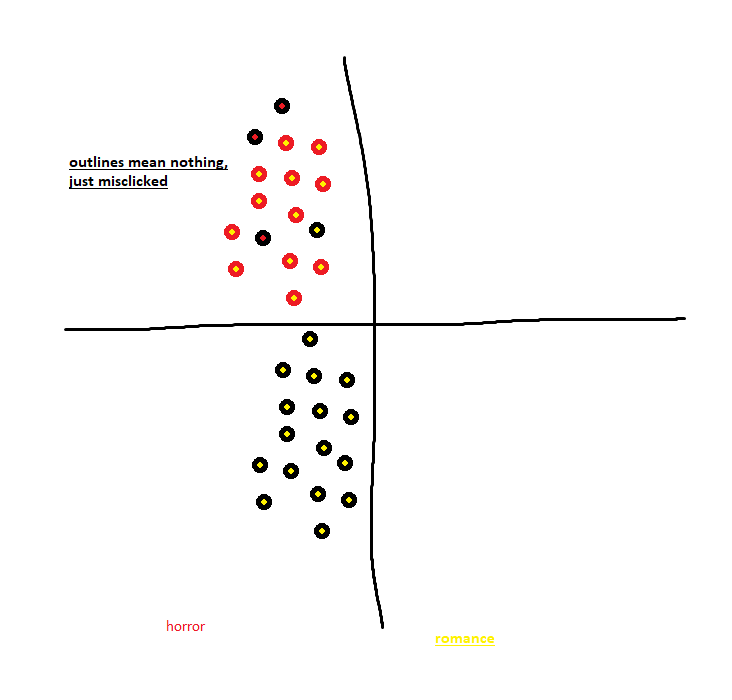
\includegraphics[width=\textwidth]{images/genres_separated.png}
	\centering
	\caption{A conceptual space of movies, where regions correspond to properties and entities are points.}\label{figure:genres_separated}
\end{figure}

\begin{table}[]
	\begin{tabular}{ll}
		& Top PPMI scoring terms                                                \\
		Example Horror Entity      & Term term term term term term term term term term term term term term \\
		Similar Horror Entity      & Term term term term term term term term term term term term term term \\
		Somewhere Inbetween Entity & Term term term term term term term term term term term term term term \\
		Romance Movie              & Term term term term term term term term term term term term term term \\
		Similar Romance movie      & Term term term term term term term term term term term term term term
	\end{tabular}
\caption{Two of the following entities: Those classified as horror, those classified as horror and romance, and those classified as romance with their associated highest value PPMI terms. We show the highest positive instances here as the representation is sparse, even though we can also expect the terms that are low scoring to be similar too.}
\label{table:PPMI_example}
\end{table}

When selecting the parameters to use for the doc2vec space when obtaining directions, we choose the one that scored the highest for its class on a Linear SVM, rather than tuning the entire process around the doc2vecs vectors.
%We use the kind of multiclass strategy as a hyper-parameter for each class-type in the grid search. We test the OneVsOne classifier method, treating each as binary problems, the OneVsRest method and the OutputCode method.
We are not able to obtain an MDS space for sentiment or doc2vec spaces for placetypes/movies.

We obtain results with just these spaces as input, and additionally results for a bag-of-words PPMI representation. These results act as our baselines for quantitative results, in addition to a Topic Model. We find results using a Linear SVM, and a Decision Tree with an unlimited depth, a depth of 3, a depth of 2, and a depth of 1. Each SVM is tuned using a grid search for the optimal C value, and whether or not to balance the classes. For all trees we attempt to find the best value between [None, 'auto', 'log2'], and additionally try differnet criterion, either the gini score or the information entropy score. In the same way as the SVM's, we include whether or not to balance the classes in the grid search.

\subsection{Word Directions}
The binary BOW representation for each word that has not been removed by the frequency cut-off is used as a target for a linear SVM, with a Semantic Space as features. We use the scikit-learn libraries LinearSVC implementation with a default C value (1.0). We balance the classes, as many of the binary BOW representations are sparse, and use the primal formulation. %Does this need to be explained more?

We obtain results for the rankings induced from these word directions on Decision Tree's limited to a depth of 3 in-order to select the best parameters when using directions for each class. The parameters that we want to determine are the type of Semantic Space, the size of the space, the frequency threshold and the score threshold. To do so, for each space-type of each size, we use a grid search to find the best frequency and score cut-offs for that sized space-type. Then, we select from these space-types and sizes the best performing one. We can understand there to be a balance between finding words which are useful for creating salient features in our clustering step without including too many words which do not. As our clustering methods are unsupervised, it is important that we try and limit the amount of junk being entered into them, despite the classifiers that use these directions typically being able to filter out those directions which are not suitable to the class. Additionally, as the vocabulary size varies from dataset to dataset, the threshold will naturally be different for each one. 

These results allow us to choose for each class, the best Semantic Space and Scoring-type for that class. For all trees we use grid search to find the best values for the criterion, either the gini score or the information entropy score, the maximum amount of features between [None, 'auto', 'log2'], and additionally, we include whether or not to balance the classes in the grid search.

%What is the importance of the space size?
%What is the importance of the space type?
%How do directions perform compared to spaces? Why?
%What kind of directions do we find for each score type?
%Why does the score type matter? What score type works best?


Next, we test single directions, attempting to find a good amount of directions to cluster and not including words which may hamper the unsupervised classification, as well as the best space-type for each domain. We found that generally, X was the best space and as expected classifiers performed better with more data, so we use 20000 as our frequency cutoff and 2000 as our score cutoff. These single directions typically overfit.


\subsection{Clustered Directions}
We continue with the optimal space and score-type chosen by our single direction experiments, and use the same frequency and score thresholds as before. We then experiment with two different clustering algorithms: Derrac and K-Means. As these algorithms select centroids from the top-scoring directions or randomly, we can expect that some clusters may not be salient features of the space. This is because top-scoring directions, e.g. for accuracy could simply infrequent terms that do not have much meaning, and these infrequehnt terms could also be randomly selected. We could use grid-search on the frequency and score cutoffs when obtaining these results in order to avoid terms that may disrupt existing clusters or form cluster centers that are not salient features of the space, but we chose a more standardized process that would rely on the parameters of the clustering algorithms and the ability of the classifiers to filter out clusters that are not informative, so as to not make a time-costly grid search a necessary part of the process.

With that in mind, we use three clustering algorithms.

Mini batch K-means, implemented by scikit-learn \footnote{https://scikit-learn.org/stable/modules/generated/sklearn.cluster.MiniBatchKMeans.html}, introduced by \cite{Sculley2010} and kmeans++ to initialize \cite{Arthur}

\subsubsection{Quantitative Results}
In Figure \ref{IntroDecisionTree}, we demonstrate how depth could affect a Decision Tree that uses salient feature-directions. 

\begin{figure}[t]
	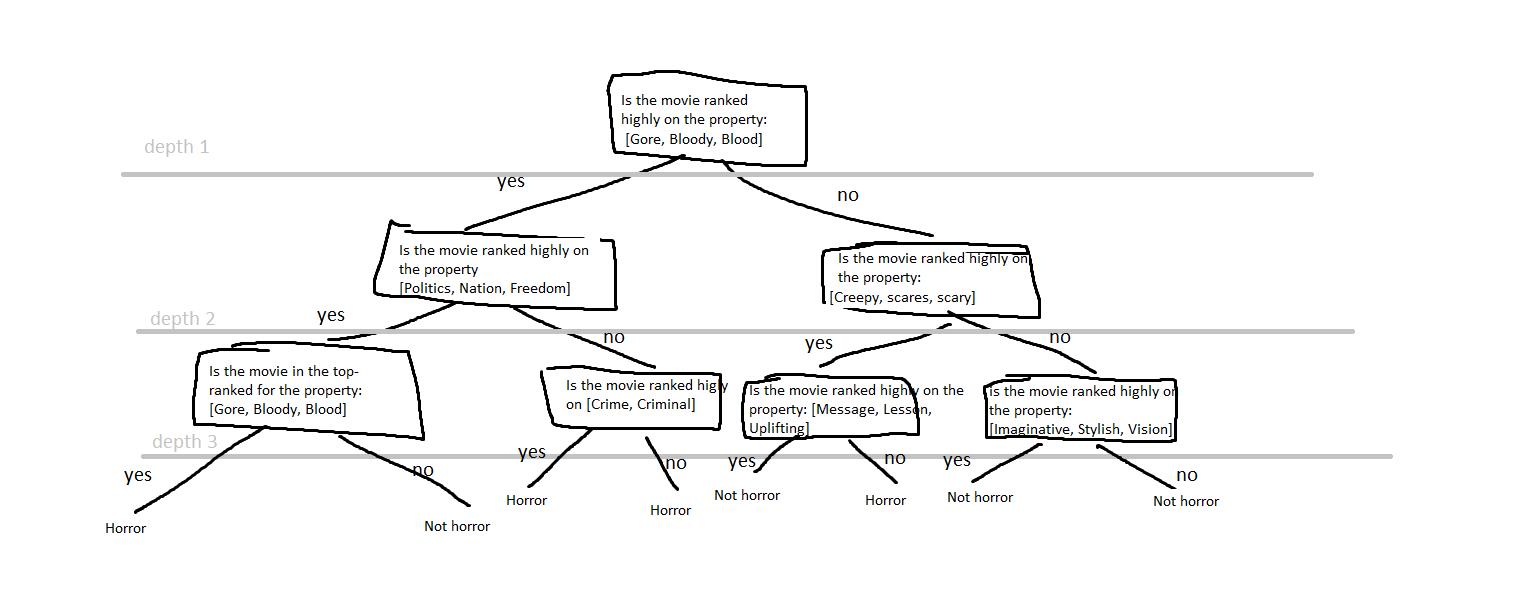
\includegraphics[width=\textwidth]{images/decisiontree.png}
	\centering
	\caption{This figure shows an example tree from one of our classifiers. Here, we can see that the model increases in complexity as it increases in depth. In this case, we end-up getting better F-score with just a depth-one tree, as the tree begins to overfit at depth three.  }\label{IntroDecisionTree}
\end{figure}

\begin{landscape}
\begin{table}[]
	\begin{tabular}{llllllllllll}
                  & Genres     &       &       & Keywords  &       &       & Ratings  &       &       &  &  \\
Movies            & D1         & D2    & D3    & D1        & D2    & D3    & D1       & D2    & D3    &  &  \\
Space             & 0.301      & 0.358 & 0.354 & 0.185     & 0.198 & 0.201 & 0.463    & 0.475 & 0.486 &  &  \\
Single directions & 0.436      & 0.463 & 0.492 & 0.230     & N/A   & N/A   & 0.466    & N/A   & N/A   &  &  \\
Clusters          & N/A        & N/A   & 0.518 & N/A       & N/A   & N/A   & N/A      & N/A   & N/A   &  &  \\
& Newsgroups &       &       & Sentiment &       &       & Reuters  &       &       &  &  \\
Rep               & 0.251      & 0.366 & 0.356 & 0.705     & 0.770 & 0.773 & 0.328    & 0.413 & 0.501 &  &  \\
Single dir        & 0.418      & 0.490 & 0.537 & 0.784     & 0.814 & 0.821 & 0.678    & 0.706 & 0.720 &  &  \\
Cluster           & 0.394      & 0.433 & 0.513 & 0.735     & 0.844 & 0.813 & 0.456    & 0.569 & 0.583 &  &  \\
& Foursquare &       &       & OpenCYC   &       &       & Geonames &       &       &  &  \\
Placetypes        & D1         & D2    & D3    & D1        & D2    & D3    & D1       & D2    & D3    &  &  \\
Rep               & 0.438      & 0.478 & 0.454 & 0.383     & 0.397 & 0.396 & 0.349    & 0.340 & 0.367 &  &  \\
Single dir        & 0.541      & 0.498 & 0.531 & 0.404     & 0.428 & 0.390 & 0.444    & 0.533 & 0.473 &  &  \\
Cluster           & 0.462      & 0.507 & 0.496 & 0.413     & 0.420 & 0.429 & 0.444    & 0.458 & 0.470 &  &  \\
	\end{tabular}\caption{Best-scoring results for each type.}
\end{table}
\end{landscape}

\section{Qualitative Results}


Make reference to the qualitative results found in the previous work here.


\subsection{Examining the differences between directions}

Investigating three potential hypothesis:
1. The ranks are more accurate, so the key directions are better represented that would contribute
2. The spaces/score-types contain unique directions that contribute to the tree directly
3. The spaces/score-types influence the rankings so that they are better represented, but are not directly used in the tree

First, we look at the best scoring directions. Then, we look at the unique directions for each space-type and score-type. The section is then followed by conclusions, and we begin to look into the clusters.

\subsection{The best-performing directions for each space type}

What are the domains that best convey the similarities and differences between different domains?

1. Find domains that act differently (perhaps one domain where a space-type that is not usually scoring high is scoring high, big differences in F1)
2. Get interesting directions from those domains

\begin{landscape}
	\begin{table}[]
		\scriptsize
		\begin{tabular}{lllll}
			\textbf{Movies} \textit{(50 MDS NDCG)}        & \textbf{Sentiment} \textit{(100 D2V NDCG)}   & \textbf{Newsgroups} \textit{(50 D2V NDCG)} 			  & \textbf{Place-types} \textit{(50 PCA Kappa)}	 						 & \textbf{Reuters} \textit{(200 MDS NDCG)}       \\
			horror (scares, scary)               & glenda (glen, matthau)         & karabag (iranian, turkiye)                 & blackcountry (listed, westmidlands)     & franklin (fund, mthly)            \\
			hilarious (funniest, hilarity)       & scarlett (gable, dalton)       & leftover (flaming, vancouver)              & ears (stare, adorable)                  & quarterly (shearson, basis)       \\
			bollywood (hindi, india)             & giallo (argento, fulci)        & wk (5173552178, 18084tmibmclmsuedu)        & spagna (espanha, colores)               & feb (28, splits)                  \\
			laughs (funnier, funniest)           & bourne (damon, cusack)         & 1069 (mlud, wibbled)                       & oldfashioned (winery, antiques)         & 22 (booked, hong)                 \\
			jokes (gags, laughs)                 & piper (omen, knightley)        & providence (norris, ahl)                   & gardening (greenhouse, petals)          & april (monthly, average)          \\
			comedies (comedic, laughs)           & casper (dolph, damme)          & celestial (interplanetary, bible)          & pagoda (hindu, carved)                  & sets (principally, precious)      \\
			hindi (bollywood, india)             & norris (chuck, rangers)        & mlud (wibbled, 1069)                       & artificial (saturation, cs4)            & 16 (creditor, trillion)           \\
			war (military, army)                 & holmes (sherlock, rathbone)    & endif (olwm, ciphertext)                   & inner (curved, rooftops)                & 1st (qtr, pennsylvania)           \\
			western (outlaw, unforgiven)         & rourke (mickey, walken)        & gd3004 (35894, intergraph)                 & celebrate (festive, celebrity)          & 26 (approve, inadequate)          \\
			romantic (romance, chemistry)        & ustinov (warden, cassavetes)   & rtfmmitedu (newsanswers, ieee)             & vietnamese (ethnic, hindu)              & 23 (offsetting, weekly)           \\
			songs (song, tunes)                  & scooby (doo, garfield)         & eng (padres, makefile)                     & cn (elevated, amtrak)                   & prior (recapitalization, payment) \\
			sci (science, outer)                 & doo (scooby, garfield)         & pizza (bait, wiretap)                      & mannequin (bags, jewelry)               & avg (shrs, shr)                   \\
			funniest (hilarious, funnier)        & heston (charlton, palance)     & porsche (nanao, mercedes)                  & falcon (r, 22)                          & june (july, venice)               \\
			noir (noirs, bogart)                 & homer (pacino, macy)           & gebcadredslpittedu (n3jxp, skepticism)     & jewish (monuments, cobblestone)         & march (31, day)                   \\
			documentary (documentaries, footage) & welles (orson, kane)           & scsi2 (scsi, cooling)                      & canon60d (kitlens, 600d)                & regular (diesel, petrol)          \\
			animation (animated, animators)      & frost (snowman, damme)         & playback (quicktime, xmotif)               & reflective (curved, cropped)            & 4th (qtr, fourth)                 \\
			adults (adult, children)             & streisand (bridget, salman)    & 35894 (gd3004, medin)                      & mason (edward, will)                    & 27 (chemlawn, theyre)             \\
			creepy (spooky, scary)               & davies (rhys, marion)          & diesel (volvo, shotguns)                   & aerialview (manmade, largest)           & 14 (borrowing, borrowings)        \\
			gay (gays, homosexuality)            & cinderella (fairy, stepmother) & evolutionary (shifting, hulk)              & shelf (rack, boxes)                     & 11 (chapter, ranged)              \\
			workout (intermediate, instruction)  & boll (uwe, belushi)            & techniciandr (obp, 144k)                   & monroe (raleigh, jefferson)             & may (probably, however)           \\
			thriller (thrillers, suspense)       & rochester (eyre, dalton)       & 8177 (obp, 144k)                           & litter (fujichrome, e6)                 & 38 (33, strong)                   \\
			funnier (laughs, funniest)           & edie (soprano, vertigo)        & shaw (medicine, ottoman)                   & streetlights (streetlamp, headlights)   & m1 (m2, m3)                       \\
			suspense (suspenseful, thrillers)    & scarecrow (zombies, reese)     & scorer (gilmour, lindros)                  & carlzeiss (f2, voigtlander)             & dlr (writedown, debt)             \\
			arts (hong, chan)                    & kramer (streep, meryl)         & xwd (xloadimage, openwindows)              & manmade (aerialview, below)             & five (years, jones)               \\
			christianity (religious, religion)   & marty (amitabh, goldie)        & ee (275, xloadimage)                       & demolished (neglected, rundown)         & bushels (soybeans, ccc)           \\
			musical (singing, sing)              & columbo (falk, garfield)       & com2 (com1, v32bis)                        & wald (berge, wildflower)                & revs (net, 3for2)                 \\
			gore (gory, blood)                   & kidman (nicole, jude)          & examiner (corpses, brass)                  & arquitetura (exposition, cidade)        & 29 (175, include)                 \\
			animated (animation, cartoon)        & juliet (romeo, troma)          & migraine (ama, placebo)                    & greyscale (highcontrast, monochromatic) & acquisition (make, usairs)        \\
			gags (jokes, slapstick)              & garland (judy, lily)           & parliament (parliamentary, armored)        & alameda (monday, marin)                 & payable (div, close)              \\          
			
		\end{tabular}
		\caption{Table}
	\end{table}
\end{landscape}


\subsection{How Domain Directions Differ}

For the single directions, arrange them by score where the highest scoring directions are at the top. For the clusters, there is no convenient way to organize them without bias, so clusters that are interesting are selected.

\subsubsection{Score Types}

There are unique directions for each different space type, each suitable to different tasks. NDCG was selected as the best score-type for Sentiment, Newsgroups, Reuters, Movies Genres, Movies Keywords in depth-3 Decision Trees. Place-types foursquare used F1-score, but the classes are very unbalanced and there are few documents. 
\begin{landscape}
\begin{table}[]
	\scriptsize
	\begin{tabular}{lllll}
		\textbf{NDCG}                     & \textbf{F1}            		     & \textbf{Accuracy}    				   & \textbf{Kappa}                     & \textbf{Common}                               \\
		gay \textit{(homosexuality, sexuality)}    & company \textit{(sell, pay)}              & kennedy \textit{(republic, elected)}             & definately \textit{(alot, awesome)}         & horror \textit{(scares, scares)}              \\
		arts \textit{(hong, chan)}                 & street \textit{(city, york)}              & bags \textit{(listened, salvation)}              & guns \textit{(gun, shoot)}                  & laughs \textit{(funnier, funnier)}            \\
		sports \textit{(win, players)}             & red \textit{(numerous, fashion)}          & summers \textit{(verge, medieval)}               & flawless \textit{(perfection, brilliantly)} & jokes \textit{(gags, gags)}                   \\
		apes \textit{(remembered, planet)}         & project \textit{(creating, spent)}        & revolve \textit{(sincerely, historian)}          & mail \textit{(reviewed, rated)}             & comedies \textit{(comedic, comedic)}          \\
		german \textit{(germans, europe)}          & mark \textit{(favor, pull)}               & locale \textit{(foster, sharply)}                & garbage \textit{(crap, horrible)}           & sci \textit{(scifi, alien)}                   \\
		satire \textit{(parody, parodies)}         & lady \textit{(actress, lovely)}           & cooler \textit{(downward, reports)}              & featurette \textit{(featurettes, extras)}   & funniest \textit{(hilarious, hilarious)}      \\
		band \textit{(rock, vocals)}               & fire \textit{(ground, force)}             & spades \textit{(ralph, medieval)}                & complaint \textit{(extra, added)}           & creepy \textit{(spooky, spooky)}              \\
		crude \textit{(offensive, offended)}       & post \textit{(essentially, purpose)}      & filmography \textit{(ralph, experiments)}        & mission \textit{(enemy, saving)}            & thriller \textit{(thrillers, thrillers)}      \\
		dancing \textit{(dance, dances)}           & heads \textit{(large, throw)}             & quentin \textit{(downward, anime)}               & ruin \textit{(wondering, heck)}             & funnier \textit{(laughs, laughs)}             \\
		restored \textit{(print, remastered)}      & water \textit{(land, large)}              & employers \textit{(finishes, downward)}          & wars \textit{(forces, enemy)}               & suspense \textit{(suspenseful, suspenseful)}  \\
		drugs \textit{(drug, abuse)}               & road \textit{(drive, trip)}               & formal \textit{(victory, kennedy)}               & prefer \textit{(compare, added)}            & gore \textit{(gory, gory)}                    \\
		church \textit{(religious, jesus)}         & brother \textit{(son, dad)}               & tube \textit{(esta, muscle)}                     & heroes \textit{(packed, hero)}              & gags \textit{(jokes, jokes)}                  \\
		sexuality \textit{(sexual, sexually)}      & party \textit{(decide, hot)}              & woefully \textit{(restless, knockout)}           & necessarily \textit{(offer, draw)}          & science \textit{(sci, sci)}                   \\
		sexually \textit{(sexual, sexuality)}      & badly \textit{(awful, poorly)}            & scientists \textit{(hilarity, locale)}           & portray \textit{(portrayed, portraying)}    & gory \textit{(gore, gore)}                    \\
		england \textit{(british, english)}        & limited \textit{(aspect, unlike)}         & overboard \textit{(civilized, cinderella)}       & critic \textit{(reviewed, net)}             & government \textit{(political, political)}    \\
		ocean \textit{(sea, boat)}                 & impression \textit{(instance, reasons)}   & rumors \textit{(homosexuality, characteristics)} & reviewed \textit{(rated, mail)}             & suspenseful \textit{(suspense, suspense)}     \\
		marry \textit{(married, marriage)}         & trip \textit{(journey, road)}             & salvation \textit{(bags, cooler)}                & saving \textit{(carry, forced)}             & frightening \textit{(terrifying, terrifying)} \\
		campy \textit{(cult, cheesy)}              & michael \textit{(producers, david)}       & actively \textit{(assassination, overcoming)}    & technical \textit{(digital, presentation)}  & military \textit{(army, army)}                \\
		christian \textit{(religious, jesus)}      & memory \textit{(forgotten, memories)}     & stretching \textit{(victory, hideous)}           & statement \textit{(exist, critical)}        & slapstick \textit{(gags, gags)}               \\
		melodrama \textit{(dramatic, tragedy)}     & james \textit{(robert, michael)}          & downward \textit{(cooler, crawling)}             & shocked \textit{(hate, warning)}            & scary \textit{(scare, scare)}                 \\
		sing \textit{(singing, sings)}             & thin \textit{(barely, flat)}              & rocked \textit{(staple, demented)}               & flying \textit{(air, force)}                & blu \textit{(unanswered, ray)}                \\
		sentimental \textit{(touching, sappy)}     & pre \textit{(popular, include)}           & affectionate \textit{(esta, muscle)}             & danger \textit{(dangerous, edge)}           & internetreviews \textit{(rhodes, rhodes)}     \\
		depressing \textit{(bleak, suffering)}     & faces \textit{(constant, unlike)}         & protest \textit{(protective, assassination)}     &                                    & cgi \textit{(computer, computer)}             \\
		evidence \textit{(investigation, accused)} & values \textit{(exception, wise)}         & confined \textit{(cooler, downward)}             &                                    & email \textit{(web, web)}                     \\
		adorable \textit{(cute, sweet)}            & unusual \textit{(odd, seemingly)}         & inhabit \textit{(quentin, drawback)}             &                                    & thrilling \textit{(thrill, exciting)}         \\
		episodes \textit{(episode, television)}    & lovers \textit{(lover, lovely)}           & latin \textit{(communities, mount)}              &                                    & web \textit{(email, email)}                   \\
		teenager \textit{(teen, teenage)}          & frame \textit{(image, effect)}            & reception \textit{(como, finishes)}              &                                    & horror \textit{(scares, scares)}              \\
		magical \textit{(fantasy, lovely)}         & mans \textit{(ultimate, sees)}            & uptight \textit{(suspensful, stalked)}           &                                    & laughs \textit{(funnier, funnier)}            \\
		health \textit{(medical, suffering)}       & efforts \textit{(generally, nonetheless)} & brink \textit{(inexplicable, freddy)}            &                                    & suspense \textit{(suspenseful, suspenseful)} 
	\end{tabular}
	\caption{Different score types}
\end{table}
\end{landscape}

\subsubsection{Comparing Space Types}

We begin by selecting the space that performed well on the genres task for the movies, with the understanding that genres as a key natural classification task will likely make use of good directions that correspond to domain knowledge. After selecting this space, we choose similarly sized spaces from the other space-types, in this case we selected the 200 dimensional MDS space as it performed the best and from there, we selected the 200 dimensional PCA space and AWV space. We also use the same score-type and frequency cut-off as the best performing space-type. In this case, the best performing type for the PCA space was 20000 frequency cutoff and NDCG, and we are comparing to 10000 frequency cutoff. This means that we are sometimes using a slightly worse performing space-type than the one we used as our final results, and that the original space has a performance advantage, but we have chosen to do so to make the results more consistent and specific. We approach these qualitative experiments with the following idea: spaces that perform better on natural domain tasks using decision trees contain unique natural directions that other spaces do not have. 

The commonalities between spaces are much more prevalent than the differences, with natural concepts of the domain being represented in all of the different space types. However, different spaces do perform better than others on natural domain tasks. In this section, we investigate why this occurs and the differences between spaces built using a standard frequency-based approach, word-vectors and doc2vec, which uses a combination of contextual information and word vectors. 

\subsubsection{Comparing MDS, AWV and PCA in the Movies domain}
\begin{landscape}
	\begin{table}[]
		\scriptsize
		\begin{tabular}{llll}
			MDS                                   & AWV                      & PCA                                     & Common                                  \\
			berardinelli \textit{(employers, distributor)} & billy \textit{(thrown, dirty)}    & amount \textit{(leaving, pick)}                  & noir \textit{(fatale, femme)}                    \\
			crawford \textit{(joan, davis)}                & brother \textit{(brothers, boys)} & fails \textit{(fit, pick)}                       & gay \textit{(homosexual, homosexuality)}         \\
			hitchcocks \textit{(hitchcock, alfred)}        & fonda \textit{(henry, jane)}      & pick \textit{(fails, fit)}                       & prison \textit{(jail, prisoners)}                \\
			warners \textit{(warner, bros)}                & building \textit{(built, climax)} & stands \textit{(fails, cover)}                   & arts \textit{(rec, robomod)}                     \\
			nuclear \textit{(weapons, soviet)}             & train \textit{(tracks, thrown)}   & surprisingly \textit{(offer, fit)}               & allens \textit{(woody, allen)}                   \\
			joan \textit{(crawford, barbara)}              & slaves \textit{(slavery, excuse)} & copyright \textit{(email, compuserve)}           & jokes \textit{(laughs, joke)}                    \\
			kidnapped \textit{(kidnapping, torture)}       &                          & length \textit{(reflect, expressed)}             & animation \textit{(animated, cartoon)}           \\
			hop \textit{(hip, rap)}                        &                          & profanity \textit{(reflect, producers)}          & sherlock \textit{(holmes, detective)}            \\
			kung \textit{(martial, jackie)}                &                          & compuserve \textit{(copyright, internetreviews)} & western \textit{(westerns, wayne)}               \\
			ballet \textit{(dancers, dancer)}              &                          & talents \textit{(admit, agree)}                  & songs \textit{(song, lyrics)}                    \\
			gambling \textit{(vegas, las)}                 &                          & admit \textit{(agree, talents)}                  & comedies \textit{(comedic, laughs)}              \\
			alcoholic \textit{(drunk, alcoholism)}         &                          & developed \textit{(introduced, sounds)}          & workout \textit{(exercise, challenging)}         \\
			waves \textit{(surfing, wave)}                 &                          & intended \textit{(bother, werent)}               & laughs \textit{(funnier, hilarious)}             \\
			jaws \textit{(jurassic, godfather)}            &                          & constantly \textit{(putting, sounds)}            & drug \textit{(drugs, addict)}                    \\
			jungle \textit{(natives, island)}              &                          & tired \textit{(anymore, mediocre)}               & sci \textit{(science, fiction)}                  \\
			employers \textit{(berardinelli, distributor)} &                          & produced \textit{(spoiler, surprising)}          & documentary \textit{(documentaries, interviews)} \\
			pot \textit{(weed, stoned)}                    &                          & involving \textit{(believes, belief)}            & students \textit{(student, schools)}             \\
			canadian \textit{(invasion, cheap)}            &                          & anymore \textit{(continue, tired)}               & thriller \textit{(thrillers, suspense)}          \\
			murphy \textit{(eddie, comedian)}              &                          & leaving \textit{(fit, pick)}                     & allen \textit{(woody, allens)}                   \\
			comics \textit{(comedian, comedians)}          &                          & makers \textit{(producers, aspects)}             & funniest \textit{(hilarious, laughing)}          \\
			kidnapping \textit{(kidnapped, torture)}       &                          & introduced \textit{(developed, considered)}      & gags \textit{(jokes, slapstick)}                 \\
			subscribe \textit{(email, internetreviews)}    &                          & loses \textit{(climax, suffers)}                 & adults \textit{(children, adult)}                \\
			vegas \textit{(las, gambling)}                 &                          & negative \textit{(positive, bother)}             & animated \textit{(animation, cartoon)}           \\
			distributor \textit{(berardinelli, employers)} &                          & expressed \textit{(reflect, opinions)}           & dancing \textit{(dance, dances)}                 \\
			wave \textit{(waves, surfing)}                 &                          & mildly \textit{(mediocre, forgettable)}          & teen \textit{(teenage, teens)}                   \\
			rhodes \textit{(internetreviews, email)}       &                          & helped \textit{(putting, allowed)}               & soldiers \textit{(soldier, army)}                \\
			hippie \textit{(pot, sixties)}                 &                          & reflect \textit{(expressed, opinions)}           & indie \textit{(independent, festival)}           \\
			weed \textit{(pot, stoned)}                    &                          & opinions \textit{(reflect, expressed)}           & suspense \textit{(suspenseful, thriller)}        \\
			caribbean \textit{(pirates, island)}           &                          & frequently \textit{(occasionally, consistently)} & creepy \textit{(scary, eerie)}                   \\
			eddie \textit{(murphy, comedian)}              &                          & content \textit{(agree, proves)}                 & italian \textit{(italy, spaghetti)}              \\
			sixties \textit{(beatles, hippie)}             &                          & allowed \textit{(helped, werent)}                & jews \textit{(jewish, nazis)}                    \\
			... 8 More                   		  &                          & suffers \textit{(lacks, loses)}                  & ... 1480 more               
		\end{tabular}
		\caption{ok dude}
	\end{table}
\end{landscape}

%We show terms unique to each domain type above. The terms are contextualized by finding the two closest term directions to the term. Here, we show the terms that are not duplicated in meaning for the other spaces. We can understand that the term 'gay (gays, homosexuality) has a similar meaning to the term 'homosexuality (gays, gay)' despite the term 'homosexuality' being high scored for one space, and the term 'gay' being highly scored for the other space. Almost all of the unique terms were of this variety. To demonstrate instead the unique meanings found in the individual spaces, we filter the results as follows: from the term and its associated descriptive terms found by getting the most similar terms, if those terms or any of the more similar terms occur in any of the terms or more similar terms in the space's top 1000 terms that we are comparing to, do not include those terms.

%We find that the 50-dimensional MDS space, which performs 0.04 F1 score higher on the genres task, finds many interesting and unique terms, which can potentially enable more nuanced decisions in the decision trees for classification. On the other hand, in the PCA space, we find terms that relate to metadata, and spanish language words. We argue that this means the MDS is better at finding unique interesting meanings than PCA, in the case of using a frequency-based BOW to create the representation.

%We perform the same process as above but comparing MDS and AWV, and find that the PPMI-based representations have their own metadata in the representation that is elevated. We can assume that the AWV space does not contain these metadata as there are simply not word-vectors available for these terms. Although, we also find unique terms that are likely to help performance on natural domain tasks for the MDS space, e.g. goodfellas, disgusting, swashbuckling. Interestingly, for the AWV space we find similar spanish-language terms, but also find some new concepts, in particular the 'republican' and 'yoga' directions. AWV was also originally 20,000 frequency and NDCG.

\subsubsection{Comparing PPMI representations to doc2vec}

\begin{table}[]
	\scriptsize
	\begin{tabular}{lll}
		\textbf{D2V}                                    & \textbf{MDS}                              & \textbf{Common}                                     \\
		leftover \textit({pizza, brake)}                & hi \textit({folks, everyone)}             & chastity \textit({shameful, soon)}                  \\
		wk \textit({5173552178, 18084tmibmclmsuedu)}    & looking \textit({spend, rather)}          & n3jxp \textit({gordon, gebcadredslpittedu)}         \\
		eng \textit({padres, makefile)}                 & need \textit({needs, means)}              & skepticism \textit({gebcadredslpittedu, n3jxp)}     \\
		porsche \textit({nanao, 1280x1024)}             & post \textit({summary, net)}              & anyone \textit({knows, else)}                       \\
		diesel \textit({cylinders, steam)}              & find \textit({couldnt, look)}             & gebcadredslpittedu \textit({soon, gordon)}          \\
		scorer \textit({gilmour, lindros)}              & hello \textit({kind, thank)}              & intellect \textit({soon, gordon)}                   \\
		parliament \textit({caucasus, semifinals)}      & david \textit({yet, man)}                 & please \textit({respond, reply)}                    \\
		atm \textit({padres, inflatable)}               & got \textit({mine, youve)}                & thanks \textit({responses, advance)}                \\
		cryptology \textit({attendees, bait)}           & go \textit({take, lets)}                  & email \textit({via, address)}                       \\
		intake \textit({calcium, mellon)}               & question \textit({answer, answered)}      & know \textit({let, far)}                            \\
		433 \textit({366, 313)}                         & interested \textit({including, products)} & get \textit({wait, trying)}                         \\
		ghetto \textit({warsaw, gaza)}                  & list \textit({mailing, send)}             & think \textit({important, level)}                   \\
		lens \textit({lenses, ankara)}                  & sorry \textit({guess, hear)}              & good \textit({luck, bad)}                           \\
		rushdie \textit({sinless, wiretaps)}            & heard \textit({ever, anything)}           & shafer \textit({dryden, nasa)}                      \\
		immaculate \textit({porsche, alice)}            & cheers \textit({kent, instead)}           & bobbeviceicotekcom \textit({manhattan, beauchaine)} \\
		keenan \textit({lindros, bosnian)}              & say \textit({nothing, anything)}          & dryden \textit({shafer, nasa)}                      \\
		boxer \textit({jets, hawks)}                    & number \textit({call, numbers)}           & im \textit({sure, working)}                         \\
		linden \textit({mogilny, 176)}                  & mailing \textit({list, send)}             & sank \textit({bronx, away)}                         \\
		candida \textit({yeast, noring)}                & call \textit({number, phone)}             & banks \textit({soon, gordon)}                       \\
		octopus \textit({web, 347)}                     & thank \textit({thanx, better)}            & like \textit({sounds, looks)}                       \\
		czech \textit({detectors, kuwait)}              & read \textit({reading, group)}            & shameful \textit({soon, gordon)}                    \\
		survivor \textit({warsaw, croats)}              & phone \textit({company, number)}          & could \textit({away, bobbeviceicotekcom)}           \\
		5173552178 \textit({circumference, wk)}         & mail \textit({send, list)}                & would \textit({appreciate, wouldnt)}                \\
		18084tmibmclmsuedu \textit({circumference, wk)} & doesnt \textit({isnt, mean)}              & beauchaine \textit({bobbeviceicotekcom, away)}      \\
		3369591 \textit({circumference, wk)}            & lot \textit({big, little)}                & ive \textit({seen, never)}                          \\
		mcwilliams \textit({circumference, wk)}         & thats \textit({unless, youre)}            & surrender \textit({soon, gebcadredslpittedu)}       \\
		coldblooded \textit({dictatorship, czech)}      & believe \textit({actually, truth)}        & problem \textit({problems, fix)}                    \\
		militia \textit({federalist, occupying)}        & youre \textit({unless, theyre)}           & windows \textit({31, dos)}                          \\
		cbc \textit({ahl, somalia)}                     & send \textit({mail, mailing)}             & gordon \textit({soon, gebcadredslpittedu)}         
	\end{tabular}
	\caption{Comparing an MDS sapce to a D2V space for Newsgroups, where a D2V space performed best.}
\end{table}

%The previous two experiments were conducted with the IMDB movies dataset, but the doc2vec space is not available for that dataset, as the original text corpus was not made available by the authors. Because of this, we choose to compare the PCA representation for the sentiment space and the Doc2Vec representation for the sentiment space, as these are still IMDB movie reviews, but instead with reviews as documents rather than compilations of reviews as documents, we can expect different directions to be important but still use our knowledge of movies and reviews to inform us. We take the 100 dimensional D2V space and the 100 dimensional PCA space, both of which perform best using the ndcg scoring type which we do not change.

%The assumption going into this analysis was that, in the same way that the AWV space does not contain metadata that is not present in the word-vectors, as will the Doc2Vec space not be informed especially by that metadata. Further, as in this case the D2V space outperforms the PCA space on the sentiment task, we also expect that by using word-context to produce the representation, we are able to find better sentiment information directions, for example by better understanding sarcasm. Additionally, the benefit of word-vectors is likely to play into this space in a positive way, informing the representation based on global context. 

%When looking at these directions, we can split the terms into two types. The names of things, and conceptual properties about movies. For the doc2vec space, the names largely dominate the unique terms list, which we can understand to mean that these terms used contextually and in the broader global context from the word-vectors is informative enough in the doc2vec space to be usefully represented. For the PCA space, there are still these unique names found, but there are less overall terms and it's a bit more balanced between concepts and names. 

%For some additional examples, we compare the MDS representation for the newsgroups and the Doc2Vec representation. The MDS performed best with F1, but we compare it to NDCG, as that is what the doc2vec space performs best with.


\subsection{What is the value of different score-types?}

\subsection{Producing Semantic Spaces}

We use unsupervised representation learning methods, with the intention to obtain a representation that represents all salient features of the domain and can adapt to a variety of tasks. 

For the semantic space, we compute the Positive Pointwise Mutual Information (See \ref{bg:PPMI}) scores for the Bag-Of-Words, and use that as input to a variety of different off-the-shelf dimensionality reduction algorithms. We explain these in further detail in Section \ref{ch3:Spaces}. 


\subsection{Quantitative Results}
From a domain, e.g. movie reviews, where each document is a collection of reviews for a movie, we preprocess the text such that it is converted to lower-case, and non-alphanumeric characters are removed. From here, we remove standard English stop words using the NLTK library \cite{Bird}. We show an example of a review's original and converted formats in Figure \ref{ch3:OrigAndConverted}. From this preprocessed corpus, we obtain a Bag-Of-Words where we count the frequency of each term $BOW_wf$, see \ref{background:BOW}. 

The difference between single directions and clusters is best highlighted when comparing their use in simple interpretable classifiers. In figure \ref{ch3:ComparedTrees} we demonstrate this.

1. Negative directions (e.g. church for horror)
2. Non-contextualized, non-direct ways of classifying, versus clustering which finds salient properties which almost directly correspond to these natural tasks.

%\begin{figure}[t]
%	\includegraphics[width=\textwidth]{images/ComparedTrees.png}
%	\centering
%	\caption{An example of a hyper-plane and its orthogonal direction in a toy domain of shapes. Green shapes are positive examples and red shapes are negative examples, but despite the problem being binary those closest to the hyper-plane are less defined than those further away, resulting in the orthogonal vector being a direction.}\label{ch3:ComparedTrees}
%\end{figure}




% Deeper explanation of our methodology and approach

\subsection{Interpretability Results}
